% !TEX encoding = UTF-8
% !TEX TS-program = pdflatex
% !TEX root = ../tesi.tex

%**************************************************************
\chapter{Tecnologie scelte e utilizzate}
\label{cap:Tecnologie scelte e utilizzate}
In questo capitolo seguirà un elenco delle tecnologie di riferimento adottate per la realizzazione dell'applicazione CS-Template.
\section{Frontend}
\subsection{Angular 6}
Angular è una piattaforam opensourse realizzato da Google nel 2016 che permette di creare le SPA, sfruttando i
pattern architetturali MVC e MVVM.

Le applicazioni sviluppate in Angular vengono eseguite interamente dal web browser dopo essere state scaricate dal web server. Questo comporta il risparmio di dover spedire indietro la pagina web al web-server ogni volta che c'è una richiesta di azione da parte dell'utente. Il codice generato da Angular gira su tutti i principali web browser moderni.

Ogni pagina web viene costruitta da diversi componenti. Un componente in Angular in generale è una piccola parte della view che reppressenta una specifica funzionalità(esempio la navbar).   Ogni component ha una propria logica
strutturale (scritta tramite appositi marcatori HTML), di presentazione (scritta con
appositi fogli di stile CSS oppure SCSS) e di business (scritta con il linguaggio di programmazione
TypeScript). Tutti i componenti possono comunicare tra di loro scambiandosi
oggetti, lo scambio viene fatto utilizzando diversi strumenti messi a disposizione da Angular. Oggi tale framework è alla versione 6.
\begin{figure}[!h] 
	\centering 
	
\includegraphics[width=0.4\columnwidth]{angular-logo} 
	\caption{Logo di Angular}
\end{figure}

\subsection{Angular material}
Angular material è una libreria che contiene una raccolta di componenti di Materia DesignG. Questo libreria è stata sviluppata sempre da Google e permette di realizzare delle UI molto avvanzata in maniena molto semplice. Fornendo una serie di semplici componenti(come i pulsanti, inputbox ecc) di Angular già fatta permette algli sviluppatori di risparmiare una notevole quantità di tempo. Tutti i componenti sono testati da Google garantendo cosi un corretto funzionamento.

\begin{figure}[!h] 
	\centering 
	
\includegraphics[width=0.4\columnwidth]{material}
	\caption{Logo di Material UI} 
\end{figure}
\subsection{SASS} Sass (Syntactically Awesome StyleSheets) è un'estensione del linguaggio CSS che permette di utilizzare variabili, di creare funzioni e di organizzare il foglio di stile in più file.

Il linguaggio Sass si basa sul concetto di preprocessore CSS, il quale serve a definire fogli di stile con una forma più semplice, completa e potente rispetto ai CSS e a generare file CSS ottimizzati, aggregando le strutture definite anche in modo complesso. SASS/CSS è un linguaggio utilizzato per definire la presentazione dell'applicazione. Poichè Angular Material fornisce molti componenti prefatti, questo linguaggio è utilizzato principalmente per definire il layout delle pagine. 
\begin{figure}[!h] 
	\centering 
	
\includegraphics[width=0.4\columnwidth]{sass}
	\caption{Logo di SASS}
\end{figure}

\subsection{HTML 5} L'HTML5 è un linguaggio di markup per la strutturazione delle pagine web, pubblicato come W3C Recommendation da ottobre 2014. HTML è stato usato come linguaggio per la definizione della logica strutturale del
front-end dell’applicazione. Una delle principali vantaggi di Angular sta proprio nel utilizzo di HTML pure rispetto i framework/librerie revali come React oppure Vue. 
\begin{figure}[!h] 
	\centering 
	
\includegraphics[width=0.4\columnwidth]{html} 
	\caption{Logo di HTML 5}
\end{figure}


\subsection{Typescript} TypeScript è un linguaggio di programmazione libero ed Open source sviluppato da Microsoft basato su EMCAScript 6. Esso estende la sintassi di Javscript aggiungendo il concetto di tipizzazione(interfacce, classi, enum ecc). Questo lo rende molto simile ai linguaggi di programmmazione come Java oppure C++, e diventa anche molto semplice l'applicazione di molti design pattern conosciuti. TypeScript nasce dal crescente bisogno di un linguaggio front-end per lo sviluppo di applicazioni JavaScript larga scala. Il linguaggio è nato dalla necessità di sicurezza e robustezza, sia da sviluppatori interni a Microsoft sia clienti. 
\begin{figure}[!h] 
	\centering 
	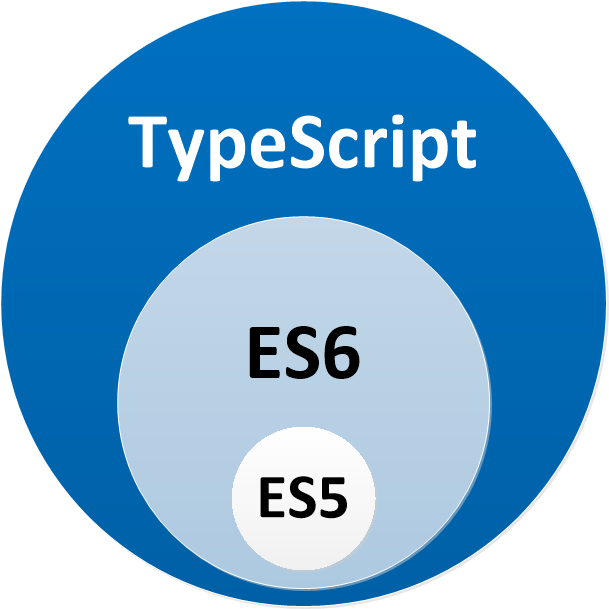
\includegraphics[width=0.4\columnwidth]{typescript} 
	\caption{Typescript rispetto ES6 e ES5}
\end{figure}

\section{Framework e le API di Zendesk}

\subsection{Zendesk Apps framework(ZAF)}
ZAF è un semplice framework sviluppato da Zendesk Inc. Viene utilizzato per realizzare le applicazione per la piattaforma Zendesk. Questo framework premette in manienra molto semplice di realizzare dei


